
\section*{Attacks}
\subsection*{Attacks in the context model}
\begin{frame}{Attacks in the context model}

\resizebox{!}{0.6\textwidth}
{
\tikzstyle{man}=[font={\Gentsroom}, scale=5]
\tikzstyle{woman}=[font={\Ladiesroom}, scale=5]

\begin{tikzpicture}[every node/.style={inner sep=0,outer sep=0}, arrows={[round]}]

\draw (-5.5,6) rectangle (2,-0.5);
\node at (-1,5.5) {Household};

\draw  (-6.5,7) [fill=white] rectangle (-4,5.5) node[pos=.5,align=center] {Home\\Production};
\draw  (-5,1.5) [fill=white] rectangle (-3.5,0) node[pos=.5,align=center] {Smart\\Meter};
\draw  (-3,4.5) [fill=white] rectangle (-1,3) node[pos=.5,align=center] {Smart\\Appliance};
\draw  (-0.5,2) [fill=white] rectangle (0.5,1) node[pos=.5,align=center] {Client};
\draw  (-9,2.5) [fill=white] rectangle (-6.5,1) node[pos=.5,align=center] {Data Hub};

\node[man] (consumer) at (1,1) {};
\node [below=0.2 of consumer] {Consumer};

\node[man] (burglar) at (-6.5,0) {};
\node [below=0.2 of burglar] {Burglar};

\node[man] (external) at (3.5,5) {};
\node [below=0.2 of external] {External};

\node[man] (power) at (-7.5,6.5) {};
\node [below=0.2 of power,align=center] {Electrical\\Company};

\node[man] (distribution) at (-7.5,4) {};
\node [below=0.2 of distribution] {Distribution};

\node[woman] (partner) at (1,4) {};
\node [below=0.2 of partner] {Partner};

\node[man] (neighbor) at (3.5,0.5) {};
\node [below=0.2 of neighbor] {Neighbor};

\draw[dashed] (-4.5,5.5) -- (-4.5,1.5);
\draw[dashed] (-6.5,1.5) -- (-6,1.5) -- (-6,1) -- (-5,1);
\draw[dashed] (-3.5,1) -- (-2.5,1) -- (-2.5,1.5) -- (-0.5,1.5);
\draw[dashed] (-2.5,3) -- (-2.5,2.25) -- (-4,2.25) -- (-4,1.5);

\draw<1,2>[ultra thick, red, -{Stealth[scale=1.2]}, bend right=90] (power) to[out=-10,in=190] (consumer);
\draw<1,2>[ultra thick, red, -{Stealth[scale=1.2]}, bend right] (consumer) to[out=-10,in=190] (power);

\draw<1,3>[ultra thick, red, -{Stealth[scale=1.2]}] (neighbor) -- (consumer);
\draw<1,3>[ultra thick, red, -{Stealth[scale=1.2]}] (partner) -- (consumer);
\draw<1,3>[ultra thick, red, -{Stealth[scale=1.2]}] (burglar) -- (consumer);

\draw<1,4>[ultra thick, red, -{Stealth[scale=1.2]}] (external) -- (consumer);


\end{tikzpicture}
}
\end{frame}

\begin{frame}{Consumer $\iff$ Electrical Company}

\resizebox{!}{0.6\textwidth}
{
\tikzstyle{man}=[font={\Gentsroom}, scale=5]
\tikzstyle{woman}=[font={\Ladiesroom}, scale=5]

\begin{tikzpicture}[every node/.style={inner sep=0,outer sep=0}, arrows={[round]}]

\draw (-5.5,6) rectangle (2,-0.5);
\node at (-1,5.5) {Household};

\draw  (-6.5,7) [fill=white] rectangle (-4,5.5) node[pos=.5,align=center] {Home\\Production};
\draw  (-5,1.5) [fill=white] rectangle (-3.5,0) node[pos=.5,align=center] {Smart\\Meter};
\draw  (-3,4.5) [fill=white] rectangle (-1,3) node[pos=.5,align=center] {Smart\\Appliance};
\draw  (-0.5,2) [fill=white] rectangle (0.5,1) node[pos=.5,align=center] {Client};
\draw  (-9,2.5) [fill=white] rectangle (-6.5,1) node[pos=.5,align=center] {Data Hub};

\node[man] (consumer) at (1,1) {};
\node [below=0.2 of consumer] {Consumer};

\node[man] (burglar) at (-6.5,0) {};
\node [below=0.2 of burglar] {Burglar};

\node[man] (external) at (3.5,5) {};
\node [below=0.2 of external] {External};

\node[man] (power) at (-7.5,6.5) {};
\node [below=0.2 of power,align=center] {Electrical\\Company};

\node[man] (distribution) at (-7.5,4) {};
\node [below=0.2 of distribution] {Distribution};

\node[woman] (partner) at (1,4) {};
\node [below=0.2 of partner] {Partner};

\node[man] (neighbor) at (3.5,0.5) {};
\node [below=0.2 of neighbor] {Neighbor};

\draw[dashed] (-4.5,5.5) -- (-4.5,1.5);
\draw[dashed] (-6.5,1.5) -- (-6,1.5) -- (-6,1) -- (-5,1);
\draw[dashed] (-3.5,1) -- (-2.5,1) -- (-2.5,1.5) -- (-0.5,1.5);
\draw[dashed] (-2.5,3) -- (-2.5,2.25) -- (-4,2.25) -- (-4,1.5);

\draw[ultra thick, red, -{Stealth[scale=1.2]}, bend right=90] (power) to[out=-10,in=190] (consumer);
\draw[ultra thick, red, -{Stealth[scale=1.2]}, bend right] (consumer) to[out=-10,in=190] (power);


\end{tikzpicture}
}
\end{frame}


\begin{frame}{Consumer $\iff$ Electrical Company}
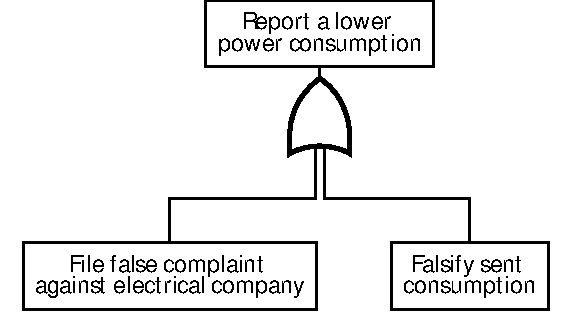
\includegraphics[width=1.1\textwidth]{graphics/consumer.pdf}

\end{frame}

\begin{frame}{Consumer $\iff$ Electrical Company}
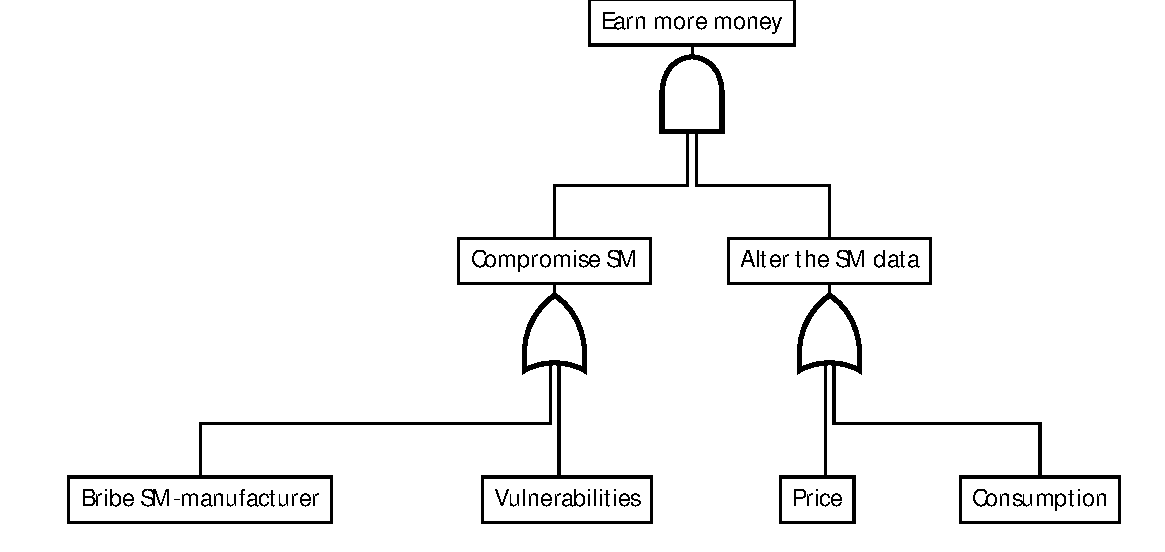
\includegraphics[width=\textwidth]{graphics/electrical_company_vs_consumer.pdf}

\end{frame}

\subsection*{Attacks from the vicinity}
\begin{frame}{Attacks from the vicinity}

\resizebox{!}{0.6\textwidth}
{
\tikzstyle{man}=[font={\Gentsroom}, scale=5]
\tikzstyle{woman}=[font={\Ladiesroom}, scale=5]

\begin{tikzpicture}[every node/.style={inner sep=0,outer sep=0}, arrows={[round]}]

\draw (-5.5,6) rectangle (2,-0.5);
\node at (-1,5.5) {Household};

\draw  (-6.5,7) [fill=white] rectangle (-4,5.5) node[pos=.5,align=center] {Home\\Production};
\draw  (-5,1.5) [fill=white] rectangle (-3.5,0) node[pos=.5,align=center] {Smart\\Meter};
\draw  (-3,4.5) [fill=white] rectangle (-1,3) node[pos=.5,align=center] {Smart\\Appliance};
\draw  (-0.5,2) [fill=white] rectangle (0.5,1) node[pos=.5,align=center] {Client};
\draw  (-9,2.5) [fill=white] rectangle (-6.5,1) node[pos=.5,align=center] {Data Hub};

\node[man] (consumer) at (1,1) {};
\node [below=0.2 of consumer] {Consumer};

\node[man] (burglar) at (-6.5,0) {};
\node [below=0.2 of burglar] {Burglar};

\node[man] (external) at (3.5,5) {};
\node [below=0.2 of external] {External};

\node[man] (power) at (-7.5,6.5) {};
\node [below=0.2 of power,align=center] {Electrical\\Company};

\node[man] (distribution) at (-7.5,4) {};
\node [below=0.2 of distribution] {Distribution};

\node[woman] (partner) at (1,4) {};
\node [below=0.2 of partner] {Partner};

\node[man] (neighbor) at (3.5,0.5) {};
\node [below=0.2 of neighbor] {Neighbor};

\draw[dashed] (-4.5,5.5) -- (-4.5,1.5);
\draw[dashed] (-6.5,1.5) -- (-6,1.5) -- (-6,1) -- (-5,1);
\draw[dashed] (-3.5,1) -- (-2.5,1) -- (-2.5,1.5) -- (-0.5,1.5);
\draw[dashed] (-2.5,3) -- (-2.5,2.25) -- (-4,2.25) -- (-4,1.5);


\draw[ultra thick, red, -{Stealth[scale=1.2]}] (neighbor) -- (consumer);
\draw[ultra thick, red, -{Stealth[scale=1.2]}] (partner) -- (consumer);
\draw[ultra thick, red, -{Stealth[scale=1.2]}] (burglar) -- (consumer);

\draw[ultra thick, red, -{Stealth[scale=1.2]}] (external) -- (consumer);


\end{tikzpicture}
}
\end{frame}

\begin{frame}{Attacks from the vicinity}
  Actors attacking the consumer have similar attack structure
\center
  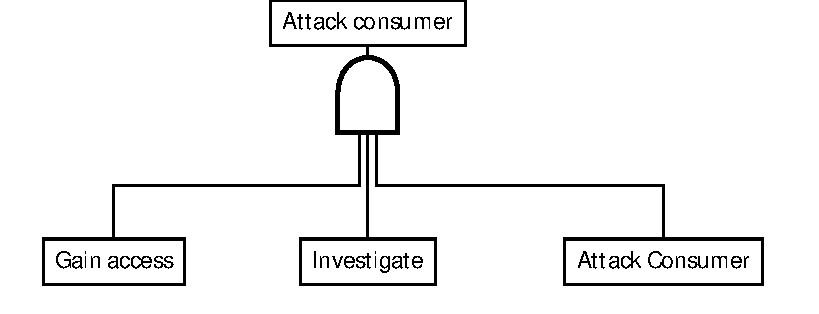
\includegraphics[width=0.7\textwidth]{graphics/common_attack.pdf}
\end{frame}

\begin{frame}{Gain access}
  \begin{block}{Accessing smart meter}
    \begin{itemize}
      \item Compromise Smart Meter
      \begin{itemize}
        \item Obtain password
        \item Bribe Smart Meter manufacturer
        \item Exploit vulnerabilities
      \end{itemize}
      \item Compromise Client
      \begin{itemize}
        \item Malware
        \item Steal Client
        \item Extract data
      \end{itemize}
      \item Install ECM
    \end{itemize}
  \end{block}
\end{frame}

\begin{frame}{Gain access}
  \begin{block}{Obtaining data }
    \begin{itemize}
      \item Buy power consumption date
      \begin{itemize}
        \item From 3rd party
        \item From the consumer
      \end{itemize}
      \item Obtain power consumption data
      \begin{itemize}
        \item Through client app
        \item Through appliance
      \end{itemize}
    \end{itemize}
  \end{block}
\end{frame}

\begin{frame}{Investigate}
  \begin{block} {When is the consumer home?}
      \begin{itemize}
        \item Look through windows
        \item Use neighborhood signals
        \item Observe physical area
        \item Device status
        \item Device schedule
      \end{itemize}
  \end{block}

  \begin{block}{What is the consumer doing?}
    \begin{itemize}
      \item Device status
      \item Turn devices on/off
    \end{itemize}
\end{block}
\end{frame}

\begin{frame}{Investigate}
    \begin{block}{What does the consumer own?}
    \begin{itemize}
      \item Device signatures
      \item Connected devices
    \end{itemize}
  \end{block}

  \begin{block}{What behavioural patterns do the consumer practice?}
    \begin{itemize}
      \item Power consumption analysis
      \item Device schedule
    \end{itemize}
  \end{block}
\end{frame}

\begin{frame}{Attack Consumer}
    \begin{block}{Direct attacks}
      Objective:
      \begin{itemize}
        \item Break in
        \item Remove annoyances
        \item Get revenge
      \end{itemize}
      Means:
      \begin{itemize}
        \item Control devices
        \item Change device schedules
      \end{itemize}
    \end{block}
\end{frame}


\begin{frame}{Attack Consumer}
  \begin{block}{Indirect attacks}
    \begin{itemize}
      \item Create consumer profile
      \item Sell data
      \item Turn off power
    \end{itemize}
  \end{block}
\end{frame}

\begin{frame}{Classification of attacks}
  The attacks can be divided into three groups
  \begin{itemize}
    \item Attacks against the privacy of the consumer
    \item Attacks on security protocols
    \item Data manipulation
  \end{itemize}
\end{frame}

\begin{frame}{Privacy}
  \begin{block}{Getting information}
    \begin{itemize}
      \item Power consumption
      \item Analyze Device signatures
    \end{itemize}
  \end{block}

  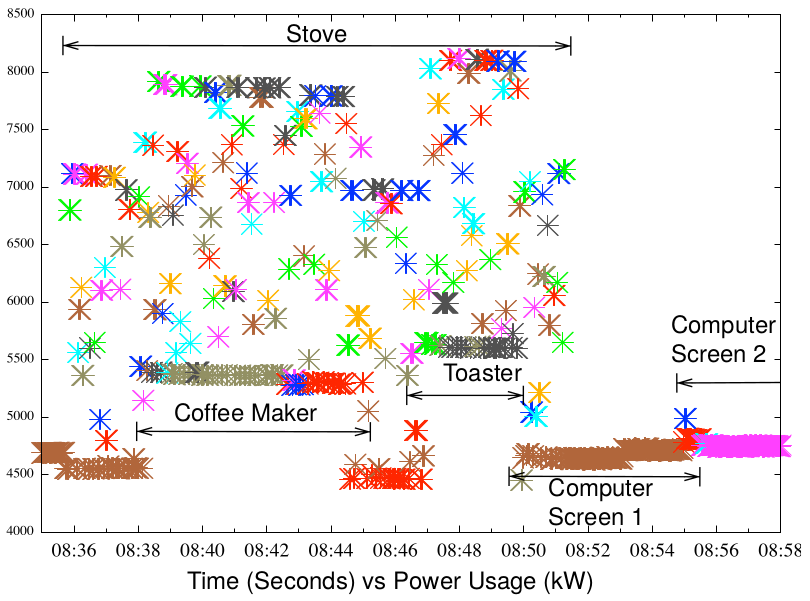
\includegraphics[width=0.7\textwidth]{graphics/detailed.png}
\end{frame}

\begin{frame}{Privacy}
  \begin{block}{Analyzing the information}
    \begin{itemize}
      \item Possible goods
      \item What is being used?
      \item Is consumer home?
      \item Owned appliance brands
    \end{itemize}
\end{block}

\end{frame}

\begin{frame}{Protocol}
\begin{block}{Issues}
  \begin{itemize}
    \item Vulnerabilities in any communication protocol compromises security
    \item Chosen protocols need to fit both hardware and security requirements
  \end{itemize}
\end{block}

\begin{block}{Security Requirements}
  \begin{itemize}
    \item Encryption
    \item Authentication
    \item Privacy
  \end{itemize}
\end{block}

\end{frame}


\begin{frame}{Data Manipulation}
  \begin{block}{Multiple Data Representations}
  \begin{itemize}
    \item Data stored on the smart meter
    \begin{itemize}
      \item Firmware
    \end{itemize}
    \item Data sent from the smart meter
    \begin{itemize}
      \item DPA
    \end{itemize}
    \item Data shown in app
    \begin{itemize}
      \item Forged apps
    \end{itemize}
  \end{itemize}
\end{block}
\end{frame}
